%-----------------------------------------------------------------------------%
\section{Results}

In all cases the group boundaries were $G = []$.
The group scalar fluxes are recovered from the angle-dependant flux by the quadrature rule ().

The first result demonstrates the discontinuous nature of the solution approximation.  Neutrons are introduce traveling from left to right with initial energy $1e10eV$.

\begin{figure}[!htbp]
\centering
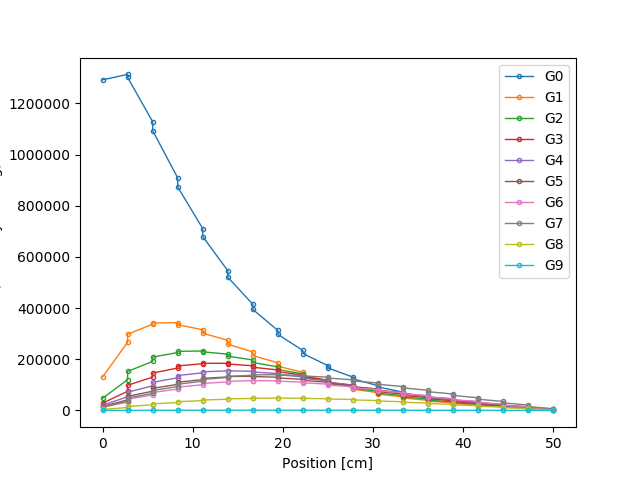
\includegraphics[width=12cm]{results/scflux_graphite_beam_1.png}
\caption{Group scalar fluxes for a high energy beam incident on a graphite block. The $y$ axis units are in $n/cm^2s$}
\label{single_ele}
\end{figure}